\chapter{Backend}


\section{Benennungen}
Folgend einige Begriffe, die häufig verwendet werden.
\begin{description}
\item[Multi-Peer]
Ein Multi-Peer ist ein Peer, welcher gleichzeitig Verbindungen zu mehreren anderen Peers pflegt.

\item[Single-Peer]
Ein Single-Peer ist ein Peer, welcher nur eine Verbindung zu einem anderen Peer pflegt.

\item[ControlPeer]
Der ControlPeer ist in diesem Projekt ein Peer, welcher Steuereingaben von dem Spieler annimmt und an den OutputClient sendet.

\item[OutputClient]
Der OutputClient ist in diesem Projekt ein Peer, welcher die Steuerangaben von den ControlPeer zugesendet bekommst und diese auswertet.
\end{description}



\section{Kommunikation}

\subsection{Zeitkritische Informationen}
Als zeitkritisch werden Informationen eingestuft, sofern sie die direkten 
Eingaben eines Peers, hier der ControlClients, und eventuelles Feedback eines anderes Peers, hier des OutputClient, betreffen. 
Da es sich bei diesem Projekt um ein Reaktionsspiel handelt, müssen diese Daten zeitnah von Sender 
zu Empfänger gelangen. Solch eine Relation ist nur über eine Peer-to-Peer 
Verbindung unter Verwendung von UDP zu realisieren.



\subsection{Möglichkeit 1: Predefined Packages 'rtc.io'}
Der NodeJS Server wird als Verbindungsserver für die Etablierung einer 
Peer-to-Peer Verbindung zwischen ControlClients und OutputClient genutzt. Als 
Technik wird konkret WebRTC eingesetzt. Auf dem NodeJS-Server wird das Package 
"rtc-switchboard" eingesetzt, welches eine Grundlage für einen  
Signalisierungsserver ist. Die Clients nutzen "rtc-quickconnect" um neues 
Channels anzufordern und eine Peer-to-Peer Verbindung zu etablieren.

\subsubsection{Vorteile}
\begin{itemize}
\item
Leichtere Implementierung, da alle Ebenen der Kommunikation bereits abgedeckt 
wurden und nur noch semantisch auf Informationen eingegangen werden muss.
\end{itemize}

\subsubsection{Nachteile}
\begin{itemize}
\item
Durch Generalisierung ein deutlicher Overhead.

\item
Status ist offiziell noch 'unstable'.
\end{itemize}



\subsection{Möglichkeit 2: Abstrakte WebRTC implementation 'WebRTC'}
Wie auch bei Möglichkeit 1 wird der NodeJS-Server als Verbindungsserver genutzt. 
Jedoch muss auf Client-Seite, also für OutputClient und ControlClient, eine 
eigene Signalling Implementation stattfinden. Es wird eine viel abtraktere 
Schicht genutzt.

\subsubsection{Vorteile}
\begin{itemize}
\item
Da die genutzen Packages nur eine Grundlage bilden, ist eine spezialisierte 
Implementierung möglich.
\end{itemize}

\subsubsection{Nachteile}
\begin{itemize}
\item
Implementierungsaufwand deutlich höher.

\item
Spezialisierung für dieses Projekt eventuell nicht nötig.

\item
Status ist offiziell noch 'unstable'.
\end{itemize}



\subsection{Möglichkeit 3: Socket.io-P2P}
Das Package Socket.io bietet auch selber eine Peer-to-Peer lösung auf WebRTC 
Basis. Hierbei wird eine Spezielle Art eines Sockets genutzt, welche wie ein 
normaler WebSocket agiert, bis ein Upgrade durchgeführt wird und die Clients nun 
direkt miteinander Kommunizieren.

\subsubsection{Vorteile}
\begin{itemize}
\item
Das Signalling und die P2P Kommunikation können mit einem Package geregelt 
werden.

\item
Variabel kann die Kommunikation über den Server, oder P2P ablaufen.

\item
Signalling events werden von Client-Server Kommunikation direkt zu P2P 
übernommen.
\end{itemize}

\subsubsection{Nachteile}
\begin{itemize}
\item
Wenig Einfluss auf die Upgrade-Mechanismen.

\item
Teils sehr instabil.
\end{itemize}



\subsection{Möglichkeit 4: Eigenes Kommunikationsmodul}
Aus Basis der WebRTC Standartimplementierung von den Browsern, kann eine eigene Schicht entwickelt werden, welche den Kommunikatinsaufbau (das Signalling) und die Kommunikationsabläufe regelt. 
Dies müsste auf einer generischen Basis geschehen um allen Anforderungen des Programmes gerecht zu werden.

\subsubsection{Vorteile}
\begin{itemize}
\item
Volle Kontrolle über Signalling und Verwaltungsabläufe der Verbindungen.

\item
Möglichkeit für schnelle Anpassungen.

\item
Unabhängigkeit gegenüber anderen Entwicklern.
\end{itemize}

\subsubsection{Nachteile}
\begin{itemize}
\item
Größter Implementierungsaufwand.

\item
Risikoabschätzung nur schwer möglich.

\item
Basis-Implementationen verschieden je Browser (gleiches Problem wie bei den anderen Implementationen: rtc.io, wocket.io-P2P, etc.)
\end{itemize}



\subsection{Statusinformationen}
Für den Austausch von Statusinformationen und Signalen zwischen Peer und Server werden WebSockets genutzt.
Für den Austausch von Statusinformationen zwischen Peers wird WebRTC genutzt.
Für den Austausch von Signalen zwischen Peers werden WebSockets genutzt, wobei der Server der Verbindungs-Knotenpunkt zwischen den Peers ist.



\subsection{Fazit nach Test}
Nach und auch schon während der Entwicklung des Prototypen hat sich 
rausgestellt, dass Socket.io-P2P in der Implementierung viele Fehler aufweist.
Gleiches gilt für rtc.io.
Eine teilweise Abänderung der Module (workarounds) führt näher an das gewünschte Ergebnis, 
verursacht aber intern wieder mehr Fehler und sorgt für eine inkonsistente Modulversion.



\subsection{Entscheidung}
Die eigene Implementation auf Basis des WebRTC bietet die meisten Möglichkeiten, birgt jedoch auch die meisten Risiken. 
RTC.io bietet eine Implementation die sehr gut für Prototypen geeignet ist, aber neben dem zeitunkritischen Signalling eine eigene Einheit bietet, welche eine Generalisierung des WebRTC darstellt und somit viel Overhead besitzt. 
Die P2P-Imeplementierung von Socket.io steht von der Implementierungs-Komplexität in der Mitte. 
Es bietet viele bereits bekannte Mechanismen des Client-Server Signalling über Events, welche mit einem Upgrade nun auch von Client zu Client funktionieren. 
Dagegen spricht jedoch die instabilität der P2P-Implementation von Socket.io. \\ \\

Eine eigene Implementation eines Modules auf Basis der von den Browsern gegebenen WebRTC-Schnittstelle ist die Wahl. 
Sie bietet die größtmögliche Flexibilität im Bezug auf Veränderbarkeit und Anpassung im laufenden Entwicklungszyklus. 
Als Risiko ist besonders der große Aufwand anzusehen.



\section{Eigenes Modul Kommunikation}

\subsection{Anforderungen an das eigene Modul für WebRTC}
\begin{itemize}
\item 
Es muss möglich sein, unsere ControlPeers nur mit dem DisplayPeer zu verbinden, 
nicht aber untereinander (Sterntopologie, wobei der DisplayPeer der Knoten ist).

\item
Der DisplayPeer muss zu jedem ihm zugeordneten ControlPeer verbunden sein.

\item
Es Muss auf Serverseite eine Raumlogik existieren, um die Peers zuordnen zu 
können.

\item
Das Signalling muss weiterhin über den Server stattfinden.
\end{itemize}



\subsection{Zuweisungslogik Server}
Der Server hat bezüglich der Zuweisungen für Verbindungen die Aufgabe alle 
Clients zu gruppieren. Dies soll ähnlich wie bei Socket.io über eine Raumlogik 
geschehen. Es existieren Räume, in welche die WebSockets auf dem Server (je Client 
also einer) eingeordnet werden.


Hierbei unterscheiden sich die Clients in ihrem Kommunikationsmodus:
\begin{description}
\item[Single]
Ein Client mit dem ''Single'' Modus pflegt nur eine direkte WebRTC Verbindung.

\item[Multi]
Ein Client mit dem ''Multi'' Modus pflegt mehrere direkte WebRTC Vebindungen 
gleichzeitig und agiert zwischen den ganzen Peers als "Host".
\end{description}

\begin{figure}[htH]
\centering
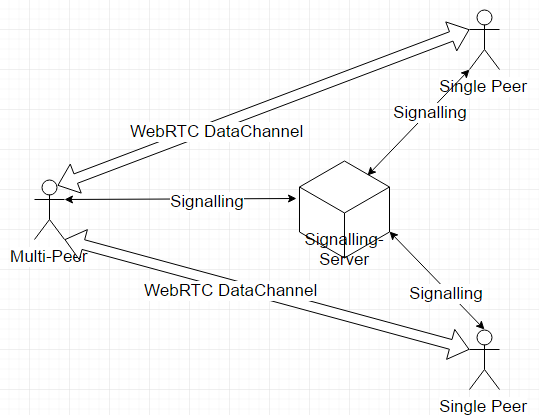
\includegraphics[width=0.9\textwidth]{backend/ConnectionBetweenPeers.PNG}
\caption{Verbindungsnetz}
\label{backfig1}
\end{figure}

In Abbildung \ref{backfig1} ist zu sehen, wie ein "Multi-Peer" mit mehreren 
"Single-Peer" gleichzeitig über WebRTC (konkret den DataChannel) kommuniziert, 
jeder einzelne "Single-Peer" aber nur mit dem einen "Multi-Peer". Zu sehen ist 
außerdem, dass das Signalling weiterhin für alle Peers über den 
Signalling-Server stattfindet, welcher hier auch gleichzeitig der WebServer ist.



\subsection{Zuweisungslogik Client (Single)}
Von nun an wird der Client der den Single Modus nutzt als "Single-Peer" 
bezeichnet.

Der Single-Peer pflegt nur eine WebRTC Verbindung, somit muss keine 
Zuweisungslogik geschehen.



\subsection{Zuweisungslogik Client (Multi)}
Von nun an wird der Client der den Multi Modus nutzt als "Multi-Peer" 
bezeichnet.


Der Multi-Peer pflegt mehrere WebRTC Verbindungen zu verschiedenen Single-Peers. 
Identifiziert werden die einzelnen Single-Peers über ein vom Server beim 
Signalling gesetztes Attribut in den Signalling Nachrichten: "from". Über dieses 
Attribut weiß der Multi-Peer von wem diese Signalling-Message kommt und kann so 
alle ankommenden Informationen diesem Single-Peer zuordnen. Somit wird unter dem 
Alias des Single-Peer ein eigenes "webRTCConnection"-Objekt verwaltet/abgelegt.
Verwendet wird hierzu ein "Assoziativer" Array, näheres in \ref{associativearray}.



\subsection{Identifizierung der Peers}
Die Peers selber erhalten in allen Signalling-Messages ein Attribut, über 
welches sie den Ursprung ermitteln können, um so Signale Peers zuordnen zu 
können. Diese \"ID'' wird vom Server vergeben und entspricht einfach nur der 
Socket ID welche die einzelnen Clients in Verbindung zum Server haben.
Da nur der Server diese ID vergibt ist diese auch eindeutig.



\section{Signalling Ablauf}
Der Ablauf ist bei den Single-Peers, sowie bei den Multi-Peers nahezu gleich.



\subsection{Anmeldung beim Server}
\begin{description}
\item[Multi-Peer]
Der Multi-Peer meldet sich beim Server mit der Bitte einen Raum zu erstellen. 
Sollte dieser Raum schon existieren ist dies ein Fehler, da in jedem Raum nur 
ein Multi-Peer existieren darf. Sollte der Raum noch nicht existieren, wird er 
erstellt und der Multi-Peer diesem zugewiesen.

\item[Single-Peer]
Der Single-Peer meldet sich beim Server mit der Bitte einen Raum zu betreten. 
Sollte dieser Raum noch nicht existieren ist dies ein Fehler, da ein Raum in 
diesem Projekt ein Spiel darstellt, ein Single-Peer (Control-Peer) aber nur 
einem bestehenden Spiel beitreten kann. Sollte der Raum bereits existieren und 
alle weiteren Spielablaufrelevanten Informationen stimmen (das Spiel darf zum 
Beispiel noch nicht angefangen haben), so tritt der Single-Peer diesem Raum bei. 
Direkt nach dem Beitreten eines Raumes, wird ein Signal an den Server gesendet, 
dass wir da sind.

\item[Server]
Sobald ein Raum existiert und ein Multi-Peer diesem zugewiesen ist, sendet jeder 
neu dazukommende Single-Peer ein Signal an den Server, dass er da ist. Dieses 
Signal wird nur an den Multi-Peer weitergeleitet.
\end{description}



\subsection{Erstes Signal}
\begin{description}
\item[Multi-Peer]
Jedes mal, wenn der Multi-Peer ein neues erstes Signal eines Single-Peers über 
den Server erhält ("hereandready"), ermittelt er seine ICE-Candidates (je nach Browser kann dieses Vorhaben eine erneute Ermittlung der Candidates, oder ein Verwenden der bereits vorher ermittelten veranlassen) und sendet 
diese an den Signalisierenden Single-Peer.
\end{description}



\subsection{ICE Candidates}
\begin{description}
\item[Multi-Peer]
Erhält ein Multi-Peer einen ICE-Candidate wird dieser der Passenden Verbindung 
hinzugefügt und löst das ''negotiationneeded''-Event aus, welches ein neues Offer 
in Form von SDP Signalisiert.

\item[Single-Peer]
Erhält ein Single-Peer einen ICE-Candidate wird dieser der akutellen 
webRTCCOnnection hinzugefügt und löst das "negotationneeded"-Event, welches ein 
neues Offer in Form von SDP Signalisiert.
\end{description}



\subsection{Aufbau über SDP}
\begin{description}
\item[Multi-Peer]
Erhält der Multi-Peer ein Offer in Form von SDP erwiedert er dieses mit einer 
Answer auch in Form von SDP und fügt die "remoteDescription" dieser 
WebRTCConnection auf Basis der Offer hinzu. Sofern dieser Vorgang Erfolg hatte 
ist eine direkte Verbindung zwischen Multi-Peer und Single-Peer entstanden.

\item[Single-Peer]
Erhält der Multi-Peer ein Offer in Form von SDP erwiedert er dieses mit einer 
Answer auch in Form von SDP und fügt die "remoteDescription" dieser 
WebRTCConnection auf Basis der Offer hinzu. Sofern dieser Vorgang erfolg hatte 
ist eine direkte Verbindung zwischen Multi-Peer und Single-Peer entstanden.
\end{description}



\subsubsection{Kommunikationskanal}
Da es sich um einfache Steuerungsdaten handelt verwenden beide Modi der Peers 
einen simplen DataChannel.



\section{Eigenes Modul: Aufbau}
\subsection{Eigenes Modul: Schnittstelle}
\begin{figure}[htH]
\centering
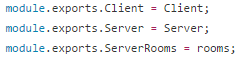
\includegraphics[width=0.9\textwidth]{backend/ModulExports.PNG}
\caption{Modul Exporte}
\label{backfig2}
\end{figure}

\begin{description}
\item[Modul.Client]
Unter Modul.Client ist eine Klassenorientierte Repräsentation des Clients zu 
finden. Es ist ein Object dieses Typs zu erzeugen.

\item[Modul.Server]
Unter Modul.Server ist eine Repräsentation des Servers zu finden. Für jeden auf 
dem Server neu Verbundenen Client muss eine neue (anonyme möglich) Instanz dieses Typs 
erstellt und dabei der WebSocket (socket.io), der mit dem Client verbunden, ist übergeben werden.

\item[Modul.ServerRooms]
Unter Modul.ServerRooms ist eine Simple Liste der derzeitigen Räume auf dem 
Server, inklusive der darin befindlichen Clients zu sehen. Diese Informationen 
sind jedoch nur auf Serverseite bei Verwendung des Modul.Server einsichtlich, 
bzw. werden nur unter Verwendung von Modul.Server aktualisiert.
\end{description}



\subsection{Eigenes Modul: Abhängigkeiten}
Das Modul ist derzeit direkt von Socket.io abhängig, von welchem es die 
WebSockets für das Signalisierungen über den Signalling-Server nutzt.



\subsection{Eigenes Modul: Struktur}
Das Modul implementiert zwei Teile. Erstens die Client-Seite. Zweitens die 
Server-Seite.



\subsubsection{Client Aufgaben}
Die Client-Implementation ist für das Frontend gedacht und nutzt alle WebRTC 
Standarts der Browserimplementationen (Mozilla, webkit und Microsoft überlagert). 
Es handelt alle Faktoren von Initiierung der Kommunikation, bis Durchführung dieser ab.



\subsubsection{Server Aufgaben}
Die Server-Implementation kümmert sich auf Server-Seite um die Einhaltung von 
Kommunikations-Standarts, die Zuweisung von Signalen und die Gruppierung vieler 
Peers.



\section{Eigenes Modul: Generischer Ansatz}

\subsection{Generische Anforderung}
Als Anforderung gilt, dass die Implementierung des Moduls von unserer Nutzung für das Ping-Pong Projekt entkoppelt ist. 
Dies ist als gegeben anzusehen, wenn die Implementation keine Hinweise auf dieses Projekt hinterlässt und Möglichkeiten zu Umsetzung anderer beliebiger Projekte bietet, ohne Anpassungen vornehmen zu müssen.



\subsection{Generische Umsetzung}
Im folgenden wird die allgemeine generische Umsetzung am Beispiel der Callbacks und Topologien gezeigt.



\subsubsection{Generische Umsetzung: Allgemein}
Im allgemeinen gibt es zwei Klassen von Peers, die ein Client nutzen kann.

\begin{quote}
  \begin{description}
  \item[Single-Peer]
  Ein Client der den Modus ''Single-Peer'' nutzt gibt damit an, dass er maximal eine direkte Verbindung zu einem anderen Peer pflegen möchte.

  \item[Multi-Peer]
  Ein Client der den Modus ''Multi-Peer'' nutzt gibt damit an, dass er eine oder mehr direkte Verbindungen zu Peers pflegen möchte.
  \end{description}
\end{quote}

Aus Kombinationen dieser Modi lassen sich verschiedene Topologien bilden. Näheres unter \ref{generictopology}.



\subsubsection{Generische Umsetzung: Callbacks}
Um jeden Nutzer dieses Moduls selbst die Verarbeitung von Ereignissen zu ermöglichen, ist die Möglichkeit gegeben, dass der Nutzer Callback-Funktionen hinterlegt, die bei gewissen autretenden Ereignissen ausgerufen werden.
Diese Ereignisse umfassen z.B:

\begin{quote}
  \begin{description}
  \item[Neue Verbindung]
  Eine neue Verbindung zu einem Peer wurde erfolgreich hergestellt.

  \item[Verbindungsverlust zu Peer]
  Eine bestehende Verbindung zu einem Peer wurde verloren.

  \item[Neue Nachricht]
  Es kam eine neue Nachricht über den DataChannel eines Peers an.
  \end{description}
\end{quote}

Weiteres zu der direkten Verwendung der Callback-Functionen unter \ref{callbacks}.



\subsubsection{Generische Umsetzung: Topologien} \label{generictopology}
Es lassen sich durch die Verwendung der zwei Modi verschiedene Topologien bilden.


\begin{quote}
  \begin{description}
  \item[one-to-one]
  Keine konkrete Topologie, aber für direkte Peer-to-Peer Verbindungen oft die gängiste Art. Beide Peers sind "Single-Peer" und pflegen jeweils nur die Verbindung zu dem anderen. 
  Siehe Abbildung \ref{backfig3}.
  \begin{figure}[htH]
  \centering
  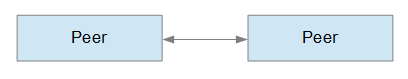
\includegraphics[width=0.9\textwidth]{backend/Topologie_1v1.PNG}
  \caption{Topologie one-to-one}
  \label{backfig3}
  \end{figure}

  \item[Stern]
  Einer der Peers agiert als Host für die anderen. Dieser Host-Peer ist der Mittelpunkt des Sternes und nutzt den Modus "Multi-Peer". Alle anderen Peers nutzen den Modus "Single-Peer" und pflegen nur die Verbindung zum Mittelpunkt (dem Host).
  Siehe Abbildung \ref{backfig4}.
  \begin{figure}[htH]
  \centering
  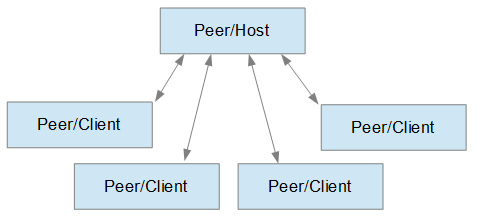
\includegraphics[width=0.9\textwidth]{backend/Topologie_4v1.PNG}
  \caption{Topologie Stern}
  \label{backfig4}
  \end{figure}

  \item[Vollvermascht]
  Alle Peers nutzen den Modus "Multi-Peer" und pflegen zu jedem anderen Peer eine direkte Verbindung.
  Siehe Abbildung \ref{backfig5}.
  \begin{figure}[htH]
  \centering
  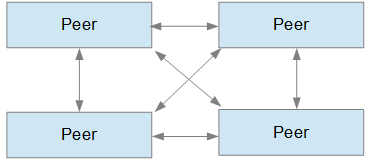
\includegraphics[width=0.9\textwidth]{backend/Topologie_ava.PNG}
  \caption{Topologie Vollvermascht}
  \label{backfig5}
  \end{figure}
  \end{description}
\end{quote}


\section{Eigenes Modul: Verwendung}

\subsection{Verwendung des Client}

\subsubsection{Abhängigkeiten}
\begin{figure}[htH]
\centering
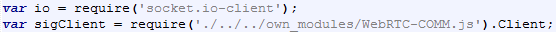
\includegraphics[width=0.9\textwidth]{backend/Modul_UserClientDependencies.PNG}
\caption{Dependencies Verwendung Client}
\label{backfig10}
\end{figure}
In Abbildung \ref{backfig10} sind die Clientseitigen Abhängigkeiten für das Modul zu sehen.
Die Client-Implementation von socket.io ''socket.io-client'' wird für das Signalling benötigt.
Zur Nutzung des Moduls muss dieses außerdem "required" werden. Hierzu wird der Pfad zu dem Modul als Parameter an das require übergeben und der Client Export genutzt.



\subsubsection{Allgemeine Verwendung}
\begin{figure}[htH]
\centering
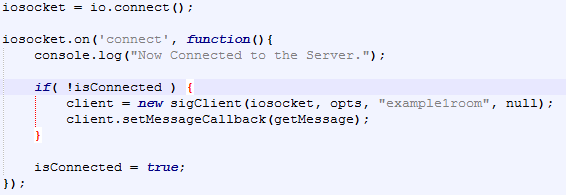
\includegraphics[width=0.9\textwidth]{backend/Modul_UserClientHowTo.PNG}
\caption{Verwendung Client}
\label{backfig11}
\end{figure}
In Abbildung \ref{backfig11} ist zu sehen, wie das Modul auf Clientseite genutzt werden kann.
Vorbedingung ist, dass wie zu sehen, eine Verbindung des socket.io WebSocket besteht.
Sobald diese besteht kann ein neues "sigClient" Objekt erstellt werden.
Diesem müssen vier Parameter übergeben werden:

\begin{description}
\item[Socket]
Der verbundene "socket.io"-Socket.

\item[Opts]
Etwaiige Optionen, alle optional. Mehr dazu unter \ref{moduleoptions}.

\item[Roomname]
Der Name des Raums, dem der Client beitreten will.

\item[Placeholder]
Ein Platzhalter für mögliche Zweitmodi.
\end{description}



\subsubsection{Nachricht Empfangen}
\begin{figure}[htH]
\centering
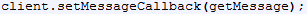
\includegraphics[width=0.9\textwidth]{backend/Modul_UserClientHowToMessageCallback.PNG}
\caption{Client Nachricht empfangen}
\label{backfig12}
\end{figure}
In Abbildung \ref{backfig12} ist zu sehen, wie eine Callback Funktion für neue Nachrichten gesetzt wird. 
Diese Funktion wird immer dann aufgerufen, wenn eine neue Nachricht empfangen wurde. Näheres zu der Struktur von Nachrichten unter \ref{messagestructure}.



\subsubsection{Nachricht Senden}
\begin{figure}[htH]
\centering
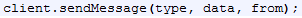
\includegraphics[width=0.9\textwidth]{backend/Modul_UserClientHowToSendMessage.PNG}
\caption{Client Nachricht senden}
\label{backfig13}
\end{figure}
In Abbildung \ref{backfig13} ist zu sehen, wie eine Nachricht versendet werden kann.
Beim Versenden einer Nachricht sind zwei Parameter von relevanz:

\begin{description}
\item[Type]
Der Typ der Nachricht. Vom Nutzer frei wählbar. Dient der schnellen Zuordnung.

\item[Data]
Die Nutzlast der Nachricht. Hierbei ist hervorzuheben, dass dies Nutzlast im Format eines JavaScript Objektes sein sollte. Sollte eine Verbindung mit WebRTC nicht hergestellt werden und der Backup-Modus ist aktiviert und unterstützt, kann dem Data-Objekt ein "to" Attribut hinzugefügt werden, welches die ID des Empfängers enthält um dem Server mitzuteilen, für wen diese Nachricht gedacht war.
\end{description}



\subsection{Verwendung des Server}
\subsubsection{Abhängigkeiten}
\begin{figure}[htH]
\centering
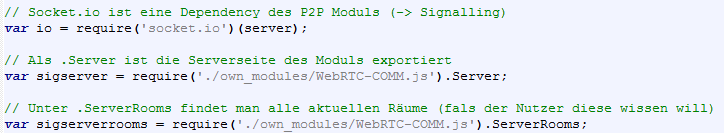
\includegraphics[width=0.9\textwidth]{backend/Modul_UserServerDependencies.PNG}
\caption{Dependencies Verwendung Server}
\label{backfig6}
\end{figure}
In Abbildung \ref{backfig6} ist zu sehen, welche Abhängigkeiten auf Serverseite bestehen.
Für das Signalling nutzt das Modul die Serverseitige Implementation von "socket.io". 
Zur Nutzung des Moduls muss dieses außerdem "required" werden. Hierzu wird der Pfad zu dem Modul als Parameter an das require übergeben und der Server Export genutzt.
Die Verwendung der ServerRooms ist optional und gibt dem Nutzer die Möglichkeit auf dem Server eine Einsicht in die derzeitigen Räume zu erlangen und über WebSockets die in diesen hinterlegt sind mit den Clients zu Kommunizieren.



\subsubsection{Konstruktor}
\begin{figure}[htH]
\centering
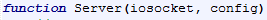
\includegraphics[width=0.9\textwidth]{backend/Modul_ServerContructor.PNG}
\caption{Server Konstruktor}
\label{backfig7}
\end{figure}
In Abbildung \ref{backfig7} ist der allgemeine Konstruktor des Moduls für Server zu sehen.



\subsubsection{Allgemeine Verwendung} \label{serveruse}
\begin{figure}[htH]
\centering
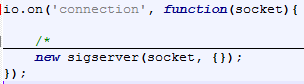
\includegraphics[width=0.9\textwidth]{backend/Modul_UserServerHowTo.PNG}
\caption{Nutzung Server}
\label{backfig8}
\end{figure}
In Abbildung \ref{backfig8} ist zu sehen, wie das Modul für Server genutzt wird. Für jeden neuen Client der sich erfolgreich mit dem Server verbunden hat muss ein neues Modul.Server Objekt erstellt werden. An dieses Modul muss der Socket (socket.io) und etwaige optionale Parameter/Optionen übergeben werden. Die Erstellung dieses Objektes führt dazu, dass Eventhandler des WebSocket für das Handling des Signalling erstellt werden und der Nutzer einem Raum zugewisen werden kann. Dies geschieht alles automatisch und intern im Modul. Der in Abbildung \ref{backfig8} zu sehende Code stellt die Minimalimplementation dar, wie sie auch im Projekt "Ping-Pong" verwendet wird. In den meisten Fällen reicht diese aus.



\subsection{Verwendung der Callbacks} \label{callbacks}
Alle wichtigen Ereignisse, welche den reibungslosen Aufbau und Betrieb der Verbindung betrifft, wird intern geregelt. Dem Nutzer des Moduls ist es jedoch möglich, eigene Callbacks zu definieren, die bei gewissen Ereignissen aufgerufen werden.
\begin{figure}[htH]
\centering
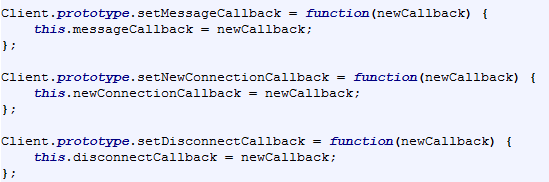
\includegraphics[width=0.9\textwidth]{backend/Modul_Callbacks.PNG}
\caption{Callbacks}
\label{backfig9}
\end{figure}
In Abbildung \ref{backfig9} sind die drei für den Nutzer wichtigsten Funktionen zum Eintragen von Callbacks zu erkennen.

\begin{description} \label{messagestructure}
\item[setMessageCallback]
Mit dieser Funktion trägt man eine Callback Funktion ein, die Falle einer neuen Nachricht aufgerufen wird. 
Die Callback Funktion wird hierbei mit drei Parametern aufgerufen:

  \begin{description}
  \item[Type]
  Dem Typen den die Nachricht hat, vergeben von dem Sender.
  
  \item[From]
  Der ID des Absenders der Nachricht.
  
  \item[Data]
  Die eigentliche Nutzlast der Nachricht. Format vom Sender bestimmt.
  \end{description}

\item[setNewConnectionCallback]
Mit dieser Funktion trägt man eine CallbackFunktion  ein, die im Falle einer neuen erfolgreichen Verbindung zu einem anderen Peer aufgerufen wird.
Die Callback Funktion wird hierbei mit einem Parameter aufgerufen:

  \begin{description}
  \item[PeerID]
  Die ID des neuen Peers.
  \end{description}
  
\item[setDisconnectCallback]
Mit dieser Funktion trägt man eine Callback Funktion ein, die im Falle des Verbindungsverlusts eines Peers aufgerufen wird.
Die Callback Funktion wird hierbei mit einem Parameter aufgerufen.

  \begin{description}
  \item[PeerID]
  Die ID des Peers, welcher die Verbindung verloren hat.
  \end{description}
\end{description}



\subsection{Verwendung der Optionen} \label{moduleoptions}
\begin{description}
\item[Client]
Beim Erstellen eines Client-Objektes können gewisse Optionen mit übergeben werden. Hierbei kann eine beliebige Anzahl dieser genutzt werden. Wird eine Option nicht genutzt, tritt ein default in Kraft (default mit = markiert):
\begin{quote}
  \begin{description}
  \item[mode (=single|multi)]
  Der Modus, den der Peer nutzen soll.
  
  \item[maxpeers (=1|1..2^3^2-1]
  Die Anzahl der maximal möglichen gleichzeitigen Verbindungen. (Relevant für "Multi-Peer")

  \item[usebackup (=false|true)]
  Die Möglichkeit der Verwendung von WebSockets als Backup. Diese option muss der Server auch Unterstzützen.
  \end{description}
\end{quote}

\item[Server]
Beim Erstellen eines Server-Objektes können gewisse Optionen mit übergeben werden.
Hierbei kann eine beliebige Anzahl dieser genutzt werden.
Wird eine Option nicht genutzt, tritt ein default in Kraft (default mit = markiert):
\begin{quote}
  \begin{description}
  \item[allowtopology_star (=true|false)]
  Sterntopologie erlauben.
  
  \item[allowtopology_1v1 (=true|false)]
  Eins zu eins "Topologie" erlauben.
  
  \item[allowtopology_ava (=false|true)]
  Vollvermaschung erlauben. Default ist false, da hierdurch auch für den Server eine große Last durch die vielen Signale entstehen kann.  
  
  \item[usebackup (=false|true)]
  Die Möglichkeit der Verwendung von WebSockets als Backup. Kann sehr Performaceintensiv werden.
  \end{description}
\end{quote}
\end{description}



\section{Eigenes Modul: Performance}
\subsection{Testbedingungen}
Diese Tests dienen ausschließlich der bewertung und Bildung eines Leistungsschemas für das Modul. Aus diesem Grund wurde der Faktor Netzwerk auf ein minimum begrenzt und nur Computer in einem LAN verwendet. Folge daraus ist, dass die Adressen dem LAN zugeordnet werden konnten und ein Routing außerhalb des LAN nicht nötig war. Eine durchschnittliche Latenz von ~1ms war gegeben (laut Anzeige, Messung erfolgte im ms Bereich). 
Ablauf eines jeden Tests:

\begin{enumerate}
\item
Es wurde ein Node.JS Server mit Minimalimplementation des Moduls gestartet. (Für Minimalimplementation siehe \ref{serveruse})

\item
Ein einzelner ''Multi-Peer'' wurde gestartet. Dieser tritt einem Testraum bei.

\item
Mit Hilfe eines kleinen Test-Programms wurde eine gewisse Anzahl an ''Single-Peer'' Sendern gestartet und via WebRTC mit dem "Multi-Peer" Host im gleichen Raum verbunden.

\item
Nachdem alle Peers erfolgreich verbunden sind wird eine Startzeit des Tests gespeichert.

\item
Die Sender fangen nun an in einer gewissen Frequenz bestimmt oft eine Nachricht an den ''Multi-Peer'' zu senden.
Die Payload dieser Nachricht besteht aus:
  \begin{description}
  \item[ID]
  Die eigene ID. Nötig da mehrere Sender auf einem System befindlich sind und nur so die zuordnung der Ergebnisse möglich ist.
  
  \item[Time]
  Ein Zeitstempel der direkt zum Sendezeitpunkt generiert wurde.
  
  \item[Index]
  Ein Index der für ID der versendeten Nachricht steht.
  \end{description}

Aus ID und Index lässt sich eine Nachricht exakt zuweisen.

\item
Empfängt der ''Multi-Peer'' eine Nachricht schickt er diese einfach direkt zum Absender zurück.

\item
Empfangt einer der ''Single-Peer'' eine Nachricht, tragen sie in ein Ergebnisobjekt den Sende- und Empfangszeitpunkt ein.

\item
Sind alle Sender mit ihren Sende-Iterationen durch und es wurde die gleiche Anzahl an Nachrichten wieder empfangen (Anzahl der Ergebnisobjekte), wird wieder ein Zeitstempel generiert.

\item
Nachdem Sende- und Empfangszyklen durch sind werden die Ergebnisobjekte ausgewertet. Dabei wird ermittelt:

  \begin{description}
  \item[Gesamtlaufzeit]
  Ermittelt aus Start- und Endzeitpunkt.
  
  \item[Gesamtzahl der Nachrichten]
  Anzahl aller empfangenen Nachrichten.
  
  \item[Minimale Delay]
  Kleinste bei einer Nachricht ermittelte Verzögerung.
  
  \item[Maximale Delay]
  Größte bei einer Nachricht ermittelte Verzögerung.
  
  \item[Durchschnittliche Delay]
  Mittelwert aller ermittelten Verzögerung.
  
  \item[Zeit pro Nachricht]
  Zeitabstand zwischen Nachrichten.
  \end{description}

\item
Wiederhole Test noch 9 mal und mittle Ergebnisse.
\end{enumerate}



\subsubsection{Erfolgskriterien}
\begin{description}
\item[Hard]
Das Harte Kriterium ist, dass das Maximale Delay nicht über der Zeit pro Nachricht liegen darf. Die Nachricht eines jeden Senders wurde also verarbeitet und beantwortet, bevor er eine neue sendet.

\item[Soft]
Das Weiche Kriterium ist, dass das durchschnittliche Delay nicht über der Zeit pro Nachricht liegen darf. Die Nachricht eines jeden Sendern wurde also in der Regel verarbeitet und beantwortet, bevor er eine neue sendet.

\item[Failed]
Sobal das weiche Kriterium nicht mehr erfüllt ist, ist ein Erfolg im allgemeinen nicht mehr gegeben. Je nach Anwendungsfall kann auch ein Failed noch ausreichend sein und es müssten speziellere Kriterien herangezogen werden.
\end{description}



\subsection{Allgemeiner Performanceaspekt} \label{associativearray}
Bei diesen Tests sollte berücksichtigt werden, dass der Verarbeitungsaufwand nach erhalt der Nachrichten sich lediglich auf das richtige weiterleiten der Nachricht beschränkt. 
Dabei wird die Nachricht an eine Callback Funktion weitergereicht und dann eine neue Nachricht an einen Peer versendet. 
Tragend für die Performance ist hier die Verwaltung der Verbindungen.
Alle Verbindungen werden in ''assoziativen'' Arrays verwaltet. Da ein ''assoziatives'' Array in JavaScript eigentlich nicht existiert, sind dies Objekte mit Attributen. 



\subsubsection{Lookup}
Je nach Browser kann das ''lookup'' verschiedene Aufwände annehmen.
Bei modernen Browsern kann von einem Worst-Case von \mathcal O\left( log_{ 2 }\left( N \right) \right) ausgegangen werden.
Bei modernen Browsern kann von einem Best-Case von \mathcal O\left( 1 \right) ausgegangen werden.
Bei älteren Browsern kann von einem Worst-Case von \mathcal O\left( N \right) ausgegangen werden.



\subsubsection{Zuweisung}
Zuweisung von Werten auf bereits bestehende Attribute von Objekten fällt unter gleichen Aufwand wie ''lookup''.
Zuweisung von Werten auf neue Attribute hat einen Aufwand von \mathcal O\left( 1 \right) im Best-Case bis \mathcal O\left( N \right) im Worst-Case je Browserimplementation. In modernen Browsern ist von \mathcal O\left( 1 \right) auszugehen.



\subsubsection{Concurrency}
Concurrency ist mit JavaScript unter den hier genutzten Techniken nicht möglich, somit müssen keine Synchronisationsmechanismen untersucht werden.




\subsection{Performance: Beispiel am Projekt}

\subsubsection{Beschreibung}
Dieser Test soll die Bedingungen des Projektes wiederspiegeln.



\subsubsection{Durchführung}
\begin{quote}
  \begin{description}
  \item[Anzahl Sender]
  Als Anzahl der Sender für die Versuche wurde festgelegt: 2, 3, 4, 6, 10, 15, 25, 50, 75, 100, 125, 150.
  
  \item[Frequenz der Nachrichten]
  Jeder Sender sendete 20 Nachrichten pro Sekunde, also alle 50ms eine Nachricht.
  
  \item[Iterationsgröße]
  Jeder Sender sendete 600 Nachrichten.
  
  \item[Folge: Nachrichtendurchsatz]
  Aus Anzahl der Sender und Frequenz entstand folgender Durchsatz(in Nachrichten/s): 40, 60, 80, 120, 200, 300, 500, 1000,     1500, 2000, 2500, 3000.
  \end{description}
\end{quote}



\subsubsection{Ergebnis}
\begin{figure}[htH]
\centering
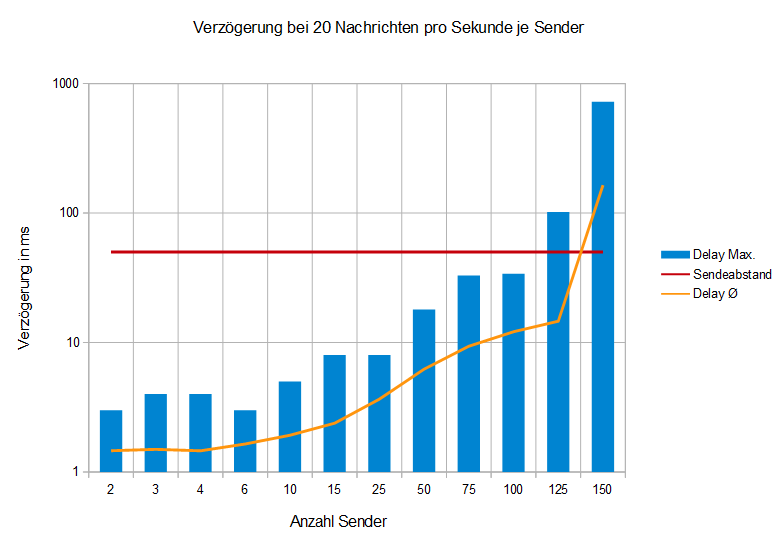
\includegraphics[width=0.9\textwidth]{backend/Diagramm_Performance_Normal.PNG}
\caption{Diagramm Performancetest Normal}
\label{backfig14}
\end{figure}
In Abbildung \ref{backfig14} ist das Ergebnis der Tests zu erkennen. 
Auf der Y-Achse ist die Verzögerung logarithmisch skaliert in ms dargestellt.
Auf der X-Achse ist die Anzahl der Sender dargestellt.
Die Balken stellen die maximale Verzögerung dar. 
Die gelbe Linie stellt die durchschnittliche Verzögerung dar.
Die rote Linie stellt die Sende-Verzögerung pro Nachricht dar.
Befindet sich ein Balken über der roten Linie ist das ''Hard''-Kriterium nicht mehr erfüllt.
Befindet sich die gelbe Linie über der roten Linie ist das ''Soft''-Kriterium nicht mehr erfüllt.



\subsubsection{Fazit}
\begin{figure}[htH]
\centering
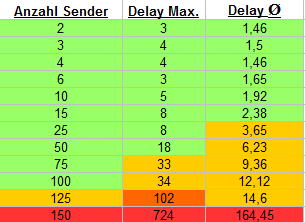
\includegraphics[width=0.9\textwidth]{backend/Tabelle_Performance_Normal.PNG}
\caption{Tabelle Performancetest Normal}
\label{backfig15}
\end{figure}
In Abbilding \ref{backfig15} ist das Ergebnis noch einmal Tabellarisch dargestellt.
Zu erkennen ist, dass das ''Hard''-Kriterium noch bis 100 Peers erfüllt ist. Dies entsrpicht einem Nachrichtendurchsatz von 2000 Nachrichten pro Sekunde. Das ''Soft''-Kriterium ist noch bis 125 Peers erfüllt. Dies entspricht einem Nachrichtendurchsatz von 2500 Nachrichten pro Sekunde. Markante Punkte:
\begin{quote}
  \begin{description}
  \item[25 Sender]
  Bei der Steigerung von 15 auf 25 Sender steigt die maximale Verzögerung nicht, jedoch die durchschnittliche Verzögerung um 53%.

  \item[75 Sender]
  Bei 75 Sendern erreicht die maximale Verzögerung zum ersten mal mehr als 50\% des ''Soft''-Kriterium.

  \item[125 Sender]
  Bei 125 Sendern ist das ''Hard''-Kriterium nicht mehr erfüllt.

  \item[150 Sender]
  Bei 150 Sendern ist das ''Soft''-Kriterium nicht mehr erfüllt.
  \end{description}
\end{quote}

Bezogen auf das Ping-Pong Projekt, welches Spieler-/Peerzahlen unter 10 nutzt, sind keine Auffälligkeiten zu erkennen und sowohl ''Soft''- als auch ''Hard''-Kriterium sind erfüllt.




\subsection{Performance: Beispiel für Chat}

\subsubsection{Beschreibung}
Folgender Test nimmt sich eine Chat-Anwendung als Beispiel.



\subsubsection{Durchführung}
\begin{quote}
  \begin{description}
  \item[Anzahl Sender]
  Als Anzahl der Sender für die Versuche wurde festgelegt: 50, 100, 150, 200, 250.

  \item[Frequenz der Nachrichten]
  Jeder Sender sendete 1 Nachricht pro Sekunde, also alle 1000ms eine Nachricht.

  \item[Iterationsgröße]
  Jeder Sender sendete 30 Nachrichten.

  \item[Folge: Nachrichtendurchsatz]
  Aus Anzahl der Sender und Frequenz entstand folgender Durchsatz(in Nachrichten/s): 50, 100, 150, 200, 250.
  \end{description}
\end{quote}



\subsubsection{Ergebnis}
\begin{figure}[htH]
\centering
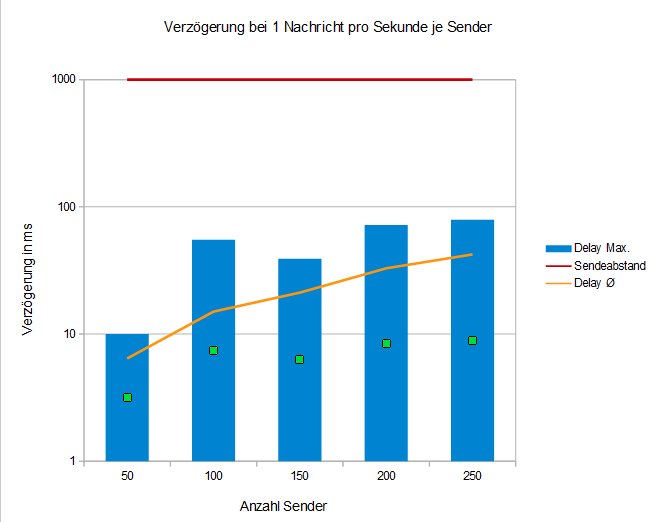
\includegraphics[width=0.9\textwidth]{backend/Diagramm_Performance_Chat.PNG}
\caption{Diagramm Performancetest Chat}
\label{backfig16}
\end{figure}
In Abbildung \ref{backfig16} ist das Ergebnis der Tests zu erkennen. 
Auf der Y-Achse ist die Verzögerung logarithmisch skaliert in ms dargestellt.
Auf der X-Achse ist die Anzahl der Sender dargestellt.
Die Balken stellen die maximale Verzögerung dar. 
Die gelbe Linie stellt die durchschnittliche Verzögerung dar.
Die rote Linie stellt die Sende-Verzögerung pro Nachricht dar.
Befindet sich ein Balken über der roten Linie ist das ''Hard''-Kriterium nicht mehr erfüllt.
Befindet sich die gelbe Linie über der roten Linie ist das ''Soft''-Kriterium nicht mehr erfüllt.



\subsubsection{Fazit}
\begin{figure}[htH]
\centering
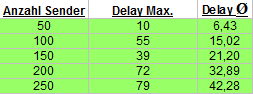
\includegraphics[width=0.9\textwidth]{backend/Tabelle_Performance_Chat.PNG}
\caption{Tabelle Performancetest Chat}
\label{backfig17}
\end{figure}
In Abbildung \ref{backfig17} ist das Ergebnis noch einmal Tabellarisch dargestellt.
Zu erkennen ist, dass auch bei 250 Sendern noch die ''Soft''- und ''Hard''-Kriterien erfüllt sind.
Ein Test mit mehr Peers stellte sich als problematisch da, da der Browser je nach Implementation bei einer großen Anzahl gleichzeitiger Verbindungen anfängt einzelne Verbindungen, die eine Weile nicht genutzt wurden, zu schließen. Dies trat auch auf, da die Initialisierungsphase des Tests diese Inaktivitätsschwälle überschritt. 
Gleichmäßige Testdurchläufe waren nicht mehr möglich.
Bester Einzeldurchlauf: 950 Peers. Inkonsistent.

Chatanwendungen auf dieser Basis stellen theoretisch keine Probleme dar.



\subsection{Performance: Beispiel extreme}
\subsubsection{Beschreibung}
Das extreme Beispiel soll zeigen, wie sich eine hohe Sendefrequenz auswirkt. Beispiel hierfür soll sein, dass Steuerdaten zu jedem Bild verarbeitet werden sollen. Hierbei markant, es soll sich um einen 144Hz Monitor handeln. (Aufgrund Rundung: 142.85Hz)



\subsubsection{Durchführung}
\begin{quote}
  \begin{description}
  \item[Anzahl Sender]
  Als Anzahl der Sender für die Versuche wurde festgelegt: 20, 25, 30, 35, 40.

  \item[Frequenz der Nachrichten]
  Jeder Sender sendete 142.85 Nachricht pro Sekunde, also alle 7ms eine Nachricht.

  \item[Iterationsgröße]
  Jeder Sender sendete 4320 Nachrichten.

  \item[Folge: Nachrichtendurchsatz]
  Aus Anzahl der Sender und Frequenz entstand folgender Durchsatz(in Nachrichten/s): 2857, 3571.25, 4285.5, 4999.75, 5714.
  \end{description}
\end{quote}



\subsubsection{Ergebnis}
\begin{figure}[htH]
\centering
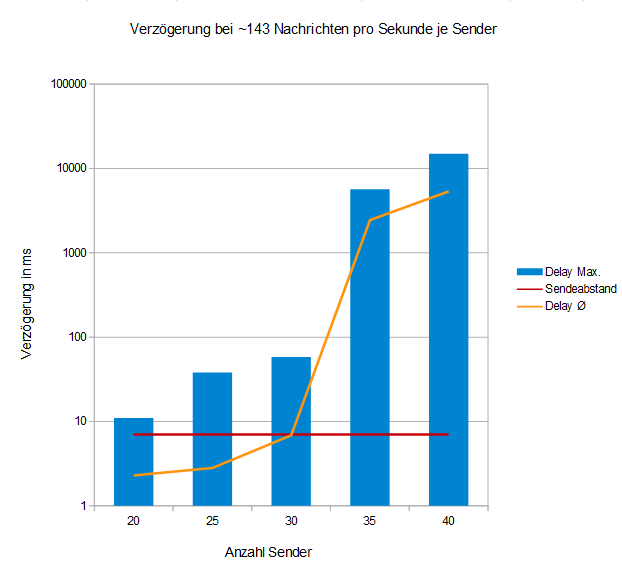
\includegraphics[width=0.9\textwidth]{backend/Diagramm_Performance_144hz.PNG}
\caption{Diagramm Performancetest 144Hz}
\label{backfig18}
\end{figure}
In Abbildung \ref{backfig16} ist das Ergebnis der Tests zu erkennen. 
Auf der Y-Achse ist die Verzögerung logarithmisch skaliert in ms dargestellt.
Auf der X-Achse ist die Anzahl der Sender dargestellt.
Die Balken stellen die maximale Verzögerung dar. 
Die gelbe Linie stellt die durchschnittliche Verzögerung dar.
Die rote Linie stellt die Sende-Verzögerung pro Nachricht dar.
Befindet sich ein Balken über der roten Linie ist das ''Hard''-Kriterium nicht mehr erfüllt.
Befindet sich die gelbe Linie über der roten Linie ist das ''Soft''-Kriterium nicht mehr erfüllt.



\subsubsection{Fazit}
\begin{figure}[htH]
\centering
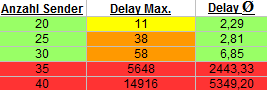
\includegraphics[width=0.9\textwidth]{backend/Tabelle_Performance_144hz.PNG}
\caption{Tabelle Performancetest 144Hz}
\label{backfig19}
\end{figure}
In Abbildung \ref{backfig19} sind die Ergebnisse noch einmal Tabellarisch dargestellt.
Zu erkennen ist, dass das ''Hard''-Kriterium schon bei 20 Sendern nicht mehr erfüllt ist.
Außerdem zu erkennen ist, dass ab 35 Sendern auch das ''Soft''-Kriterium nicht mehr erfüllt ist.

Markante Punkte:

\begin{quote}
  \begin{description}
  \item[20 Sender]
  Bei 20 Sendern ist das ''Hard''-Kriterium nicht mehr erfüllt, die durchschnittliche Verögerung aber noch sehr gut.

  \item[25 Sender]
  Im Gegensatz zu 20 Sendern, hat sich bei 25 Sendern die Maximale Verzögerung um 245\% auf 38ms erhöht. Anzeichen für einen zeitweisen Nachrichtenstau.

  \item[30 Sender]
  Im Gegensatz zu 25 Sendern, hat sich bei 30 Sendern die durchschnittliche Verzögerung um 143\% auf 6.85ms erhöht. Ein Zeichen dafür, dass immer öfter Nachrichtenstaus auftreten.

  \item[35 Sender]
  Im Gegensatz zu 30 Sendern, hat sich bei 35 Sendern die maximale Verzögerung um 9637\% auf 5648ms und die durchschnittliche Verzögrung um 35569\% auf 2443.33ms erhöht. Hierbei ist von einem Durchgängig anwachsendem Nachrichtenstau auszugehen.

  \item[40 Sender]
  Noch einmal hat sich im Gegensatz zu 35 Sendern bei 40 Sendern die Verzögerung noch einmal vervielfacht.
  \end{description}
\end{quote}

Sofern das ''Hard''-Kriterium kein muss ist, können solche Mengen an Nachrichten noch bis 30 Sender verarbeitet werden.



\section{Eigenes Modul: Möglichkeiten}

\subsection{Verwendbarkeit}
Das Modul ist wie im Projekt genutzt getestet und verwendbar. 
Es ist generisch nutzbar.
Einige zusätzliche Features, welche auch für das Projekt nicht von Relevanz waren, sind nur teilweise implementiert oder nicht getestet. 
Dies ist auf den großen Umfang eines solchen Modules zurückzuführen. \\ \\
Bei diesen teilweise implementierten Features handelt es sich um:
\begin{enumerate}
\item
Interaktiven Raumwechsel.

\item
Benutzerspezifische Sendekanäle.

\item
Echtzeit Verbindungsanalysen.
\end{enumerate}
\\ \\
Bei den nicht ausführlich getesteten Features handelt es sich um:
\begin{itemize}
\item
Topologie Eins-zu-Eins und Vollvermascht. Grund ist, dass hierfür weitere Testanwendungen nötig wären.

\item
Backup funktionalität über WebSocket. Grund ist, dass ein Test in verschiedenen Netzen noch erfolgen muss.
\end{itemize}


\subsection{Erweiterbarkeit}
\begin{itemize}
\item
Angesichts der verschiedenen möglichen Topologien gibt es für die Peers nur zwei verschiedene Verhalten. 
Entweder sie pflegen nur eine Verbindung, oder mehrere.
Da dieses Verhalten bereits modelliert ist, ist die implementation neuer Topologien auf Serverseite zu geschehen, welche die Räume verwaltet.

\item
Als Verbindungsobjekte werden unveränderte RTCPeerConnections verwendet, wodurch das hinzufügen neuer Datenkanäle ein neues Verwalungsobjekt auf Clientseite benötigen würde.
Außerdem müssten die verschiedenen Datenkanäle entweder auf mehrere Callback Funktionen gemapped werden, oder ein Parameter für die eine Callback Funktion definiert werden, welche die Datenkanäle logisch trennt.

\item
Für die Implementation von Speziellen Datenkanälen, wie z.B. Medienkanälen, muss ähnlich wie bei den normalen Datenkanälen, ein Verwaltungsobjekt geschaffen werden, und etwaiige Callback Funktionen bestimmt.

\item
Die Implementation eines Senderelays (A, B, C und D sind Peers. A sendet an D über B und C: A->B->C->D) liegt in Nutzerhand. Es müsste eine Implementation stattfinden bei dem ein Client (B und C) zwei Verbindungen herstellt. 
Dabei pflegt B jeweils eine zu A und C, C jeweils zu B und D.
Ankommende Nachrichten müssten dann an die andere Verbindung weitergereicht werden.
Diese Nutzer-Implementation könnte dann auch die Teilvermaschung ermöglichen.
\end{itemize}



\section{Fazit der Arbeit am Modul}
Die große Fehlermenge anderer Module zeigt, wie komplex ein genau definiertes Thema sein kann.
Etliche verschiedene kleine Abweichungen der Browserspezifischen WebRTC-Implementationen führen dazu, dass auf viele ''Marotten'' eingegangen werden muss.
Auch wenn dieses Modul einen bis dato guten Ansatz liefert, fehlen noch viele bereits beschriebene Features, um dieses Modul ein vollständiges nennen zu können.
Die Erstellung eines solchen Moduls ist vom Umfang her größer einzuordnen, als anfänglich erwegt. 
Viele Refactoringschritte wurden nicht durchgeführt, dar der Zeitliche Aspekt dieses Projektes dies nicht mehr zu ließ.